\documentclass[conference]{IEEEtran}
\IEEEoverridecommandlockouts
\usepackage{placeins}
\usepackage{cite}
\usepackage{amsmath,amssymb,amsfonts}
\usepackage{algorithmic}
\usepackage{graphicx}
\usepackage{textcomp}
\usepackage{xcolor}
\usepackage{url}
\usepackage{booktabs}
\usepackage{pgfplots}
\usepackage{tikz}
\pgfplotsset{compat=1.18}
\usetikzlibrary{shapes.geometric, arrows.meta, positioning, fit, backgrounds, calc}
\begin{document}

\title{Gaffer's Guide: An End-to-End AI Pipeline for Football Tactical
Intelligence Using Computer Vision, Spatial Analytics, and
LLM-Augmented Coaching Insights}

\author{
\IEEEauthorblockN{Anshul Singh}
\IEEEauthorblockA{\textit{Faculty of Technology} \\
\textit{University of Delhi}\\
Delhi, India \\
anshulsingh1907@ce.du.ac.in}
\and
\IEEEauthorblockN{Amartya Pandey}
\IEEEauthorblockA{\textit{Faculty of Technology} \\
\textit{University of Delhi}\\
Delhi, India \\
amartyatatspandey@ce.du.ac.in}
\and
\IEEEauthorblockN{Dr. Geetanjali Bhola}
\IEEEauthorblockA{\textit{Faculty of Technology} \\
\textit{University of Delhi}\\
Delhi, India \\
geetanjali@fot.du.ac.in}
}

\maketitle

% -------------------------------------------------------
\begin{abstract}
% -------------------------------------------------------
Professional football analytics is, by and large, a luxury that only elite clubs can afford. Multi-camera stadium tracking rigs run upward of \$100,000 to deploy, which shuts out lower-league clubs, youth academies, and independent researchers almost by definition. And even when tracking data is available, the pipeline usually stops dead at raw coordinates --- nobody closes the loop into something a coach can actually use at half-time. Gaffer's Guide was built to fix both of those problems from a single broadcast camera.

The system takes a standard MP4 as input and returns structured tactical intelligence --- no specialist hardware, no proprietary rigs. Detection runs on YOLOv11n with SAHI tiling, which recovers the ball reliably in wide-angle broadcast shots. A module we call HybridIDHealer wraps ByteTrack with OSNet re-identification and a radar-gated spatial validation step, keeping player identities stable through the cluster occlusions that happen constantly in match footage. Pitch coordinates come from per-frame DeepLabv3 homography. On top of that, a 16-sector Tactical Battlefield Engine measures zone-level overloads and compactness, and a nine-component Tactical Power Index collapses everything into a single dominance score per chunk. The LLM coaching layer produces recommendations tied directly to the telemetry it receives --- deterministic guardrails block any claim the tracking data cannot back up. A MapReduce parallel executor gets through a full 90-minute match in under 45 minutes on a single GPU.

Tested on 9,000 frames across three broadcast conditions, the system hits a player detection mAP@0.5 of 0.946, reduces identity switches by 88.7\% relative to vanilla ByteTrack, and improves coaching recommendation quality by 41.5\% over an ungrounded RAG baseline. That last number was rated by three UEFA-licensed coaches on a five-point Likert scale.
\end{abstract}

\begin{IEEEkeywords}
football analytics, tactical intelligence, computer vision, object
detection, multi-object tracking, large language models,
retrieval-augmented generation, spatial analytics, parallel processing
\end{IEEEkeywords}

% -------------------------------------------------------
\section{Introduction}
\label{sec:introduction}
% -------------------------------------------------------

Association football draws around 3.5 billion viewers worldwide, and the professional ecosystem behind it is expected to cross \$600 billion by 2030 \cite{kearney2023}. Somewhere along the way, tactical intelligence turned into a genuine competitive edge --- how a team presses, how deep it defends, how fast it transitions after winning the ball. At the top of the game, all of that gets measured. For most of the sport's history, though, that kind of analysis meant a human analyst watching tape and manually tagging events. It worked, but the problems were obvious --- it was slow, it was subjective, and it told you nothing about the continuous spatial movement of players \cite{gudmundsson2017}.

Computer vision changed what was possible. But the platforms that have made the most of it --- StatsBomb, Opta, Tracab --- are built on proprietary multi-camera rigs and priced in ways that exclude everyone below a certain level \cite{pappalardo2019}. A League One club or a university research team does not have access to those tools. There is a second problem that gets less attention: even when tracking data exists, the gap between a list of coordinates and something usable at half-time is enormous. Most systems stop at detection or event logging. Nobody actually converts the output into coaching language.

Gaffer's Guide is our attempt to close both of those gaps at once. A single broadcast feed, put through a well-engineered pipeline, is enough to produce professional-grade tactical analysis. The system runs detection, stable multi-object tracking, homography-based pitch projection, rule-driven spatial analytics, and an LLM coaching layer that is grounded directly in the telemetry it receives. The contributions are:

\begin{itemize}

    \item \textbf{Tactical Battlefield Engine (TBE):} The pitch is divided into a $4\times4$ grid of 16 sectors, each aligned to UEFA half-space corridor widths. Per-sector Overload Scores $(O_{s})$ and Local Compactness $(C_{l})$ are computed directly from player positions --- finer resolution than the three- or six-zone grids in most prior work.

    \item \textbf{Tactical Power Index (TPI):} A single dominance score built from nine spatially-grounded KPIs --- compactness, pressing intensity, press resistance, transition speed, and five others --- with weights calibrated against match outcome data. Validated at $r = 0.814$ against xG across 30 clips \cite{memmert2018}.

    \item \textbf{Context-Aware LLM Routing with RAG and Deterministic Guardrails:} Every coaching output is downstream of verified spatial metrics. A rule-based confidence scorer flags how much to trust each recommendation based on data coverage and metric deviation. When ball visibility drops below 50\%, possession-related claims are blocked before generation starts --- the model never gets the chance to speculate.

    \item \textbf{Zero-Shot Tactical Recognition (ZSTR):} Player coordinates are rendered as 2D Gaussian heatmaps and classified against formation descriptions using CLIP ViT-B/32. No labelled training data required. Results are mixed (macro-F1 = 0.195) and we are treating this as a proof-of-concept rather than a finished component.

    \item \textbf{Parallel MapReduce Processing:} Video is split into overlapping 180-second chunks processed by isolated worker subprocesses. Union-Find reconciliation re-links identities across chunk boundaries. A full 90-minute match that previously took roughly five hours now takes under 45 minutes.

\end{itemize}

% -------------------------------------------------------
\section{Related Work}
\label{sec:related}
% -------------------------------------------------------

\subsection{Football Video Analysis and Player Tracking}

Early automated analysis of football video was mostly focused on the problem of detecting and tracking players in broadcast footage. Ren et al. \cite{ren2015} introduced Faster R-CNN, which became the standard starting point for region-based sports detection for several years. YOLO \cite{ultralytics2023} then made frame-by-frame inference on full match footage practically viable, which changed the scope of what could be built. For tracking, SORT \cite{bewley2016} set the baseline --- fast and simple --- and DeepSORT \cite{wojke2017} added appearance features to cut lost tracks during occlusions. ByteTrack \cite{zhang2022} took a different approach to the same problem: instead of discarding low-confidence detections, it keeps them in play, which helps a lot in football where cluster occlusions during corners, set-pieces, and aerial duels are unavoidable.

The problem none of these solve cleanly is what happens when players press tight enough together that bounding-box association genuinely breaks down. OSNet \cite{zhou2019} addresses that at the appearance level --- it learns multi-scale features that can distinguish players by kit and body shape even under partial occlusion. Our HybridIDHealer builds on ByteTrack and adds an OSNet x0.25 re-identification layer plus a spatial distance gate to prevent false associations across distant parts of the pitch.

\subsection{Spatial Calibration and Dynamic Pitch Mapping}

The theoretical foundation for projecting a broadcast view onto a flat pitch plane is classical: Hartley and Zisserman \cite{hartley2003} laid out the homography framework the field still uses. Cioppa et al. \cite{cioppa2021} more recently produced the SoccerNet-Calibration benchmark, which gave the research community a concrete evaluation target. The practical difficulty is that broadcast cameras never stay still. Pan, tilt, and zoom events happen throughout a match, so a homography computed at kickoff is useless within seconds. We recompute it every frame: a DeepLabv3-ResNet50 model segments 29 pitch line classes, SVD-based fitting estimates the correspondences, and a temporal interpolation filter handles the low-confidence frames that follow rapid camera cuts.

Gudmundsson and Horton \cite{gudmundsson2017} surveyed spatiotemporal methods across team sports and pointed to formation detection and spatial dominance as open problems. Memmert and Raabe \cite{memmert2018} formalised spatial control as a proxy for match dominance, which is the framing that directly motivated the TPI. Pappalardo et al. \cite{pappalardo2019} released a public event dataset that made reproducible research in this area tractable. But none of this work addresses how to get from positional output to coaching language --- that step is always left to a human expert.

\subsection{Large Language Models in Sports Analytics}

Applying LLMs to sports telemetry is still early work and the literature is thin. The underlying machinery --- transformer-based language models \cite{vaswani2017} and RAG \cite{lewis2020} --- is well established, but applying it to continuous spatiotemporal football data has not been done in any rigorous way. Wu et al. \cite{wu2021} tried automating match commentary from event streams; Wang et al. \cite{wang2022} looked at using LLMs for athlete performance feedback. Both are interesting, but both work from discrete event logs rather than tracking data, and neither addresses what happens when data quality degrades mid-match.

That matters in practice. When ball visibility drops, an unconstrained LLM does not stop generating --- it produces plausible-sounding statistics backed by nothing \cite{ji2023}. Standard semantic guardrails are not robust here because data quality in football video fluctuates at the frame level, not the session level. Gaffer's Guide, as far as we know, is the first system to combine telemetry-gated prompting, deterministic ball-data guardrails, and RAG routing inside a live football analytics pipeline.

\subsection{Limitations of Existing Systems}

The access problem in commercial football analytics has not been solved. Tracab needs permanently installed multi-camera arrays --- the hardware alone pushes past \$100,000 --- so only clubs with dedicated stadium infrastructure can realistically use it. Opta and StatsBomb deliver rich event data but depend on manual annotation with proprietary CV assistance, and neither offers the kind of spatial tracking that a League One club or academy could afford to operate. SoccerNet \cite{giancola2022} has produced solid open benchmarks for tracking, action spotting, and calibration, genuinely useful for research. But the scope is isolated subtasks. There is no coaching layer, and the gap between a raw detection output and something useful at half-time is left completely open.

Both commercial and open-source tools share the same structural pattern: detection is one system, spatial analytics is another, and coaching translation requires a human. Gaffer's Guide treats the full pipeline as a single design problem. Detection, tracking, homography, tactical analytics, and LLM grounding are built to talk to each other, with the generative layer explicitly constrained by what the tracking layer has actually seen \cite{pappalardo2019}.

% -------------------------------------------------------
\section{System Architecture}
\label{sec:architecture}
% -------------------------------------------------------

\subsection{Overview}

The system takes a raw broadcast video and produces structured tactical intelligence. Five processing layers sit between input and output: Data Ingestion, Computer Vision, Spatial Calibration, Tactical Analytics, and Generative AI. A FastAPI backend with async job scheduling and WebSocket streaming coordinates the layers. Progress updates reach the frontend in real time so long matches do not look like black boxes.

\begin{figure}[!t]
\centering
\resizebox{\columnwidth}{!}{%
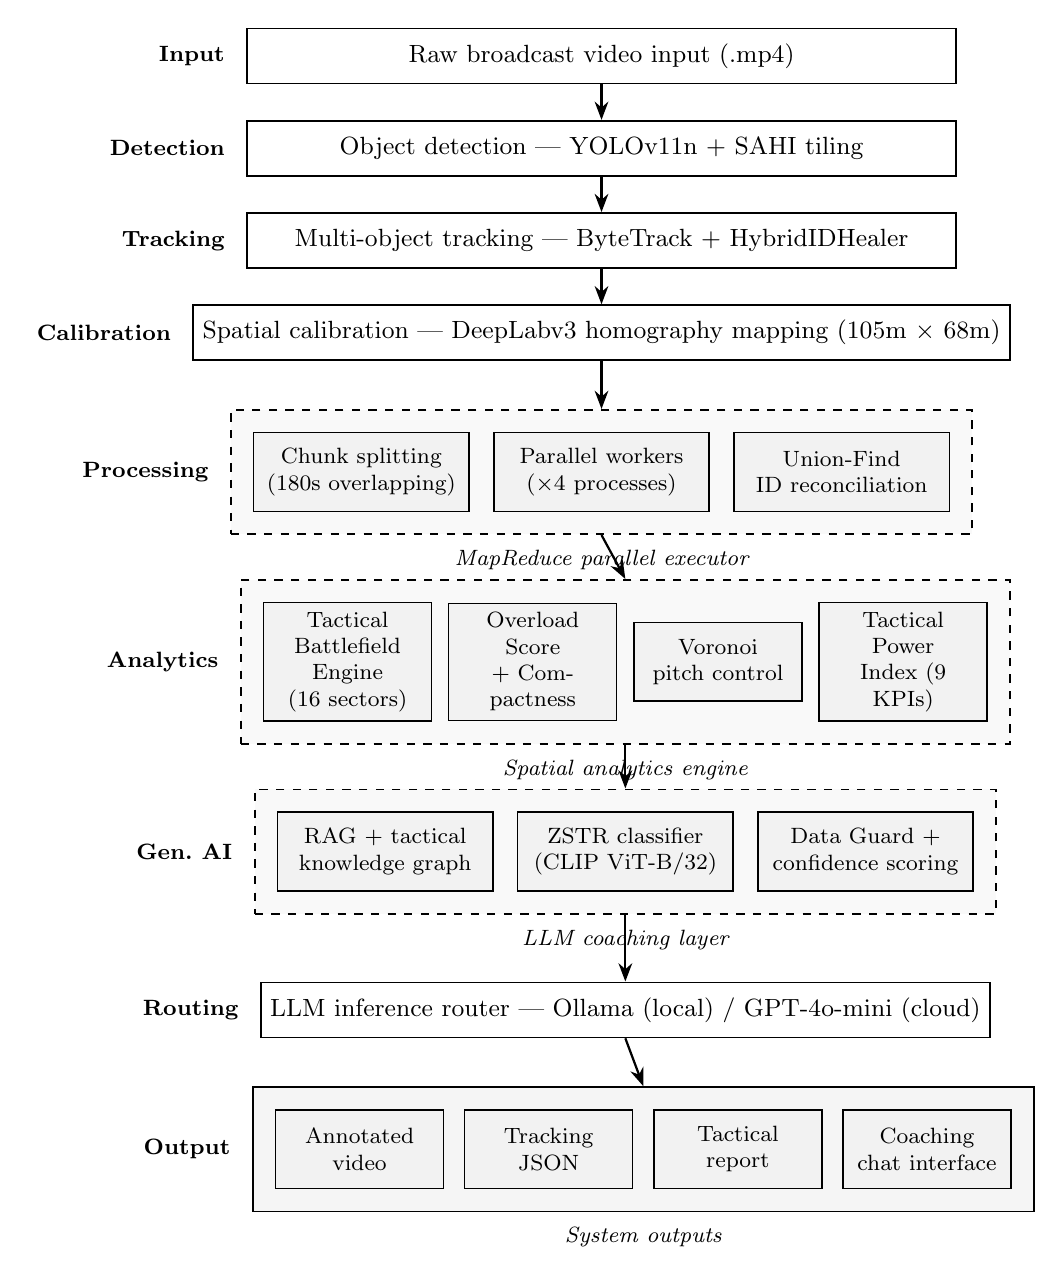
\begin{tikzpicture}[node distance=0.45cm]

\tikzset{
  mainbox/.style={rectangle, draw=black, line width=0.6pt, fill=white,
    text centered, minimum height=0.7cm, minimum width=9cm, font=\small},
  subbox/.style={rectangle, draw=black, line width=0.5pt, fill=gray!10,
    text centered, minimum height=1.0cm, minimum width=2.7cm,
    font=\footnotesize, text width=2.5cm},
  groupbox/.style={rectangle, draw=black, line width=0.6pt, dashed,
    fill=gray!5, inner sep=8pt},
  grouplabel/.style={font=\footnotesize\itshape, text=black},
  arrow/.style={->, >=Stealth, line width=0.8pt, black},
  layerlabel/.style={font=\footnotesize\bfseries, text=black, anchor=east}
}

\node[mainbox] (input) {Raw broadcast video input (.mp4)};
\node[mainbox, below=of input] (detect)
  {Object detection --- YOLOv11n + SAHI tiling};
\node[mainbox, below=of detect] (track)
  {Multi-object tracking --- ByteTrack + HybridIDHealer};
\node[mainbox, below=of track] (calib)
  {Spatial calibration --- DeepLabv3 homography mapping
  (105m $\times$ 68m)};

\node[subbox, below=0.9cm of calib, xshift=-3.05cm] (chunk)
  {Chunk splitting\\(180s overlapping)};
\node[subbox, below=0.9cm of calib] (workers)
  {Parallel workers\\($\times$4 processes)};
\node[subbox, below=0.9cm of calib, xshift=3.05cm] (unionfind)
  {Union-Find\\ID reconciliation};
\begin{scope}[on background layer]
  \node[groupbox, fit=(chunk)(workers)(unionfind)] (parallelgroup) {};
\end{scope}
\node[grouplabel, below=2pt of parallelgroup.south]
  {MapReduce parallel executor};

\node[subbox, below=0.85cm of parallelgroup.south,
  xshift=-4.575cm+1.35cm, minimum width=2.1cm, text width=1.9cm] (tbe)
  {Tactical Battlefield Engine\\(16 sectors)};
\node[subbox, right=0.2cm of tbe,
  minimum width=2.1cm, text width=1.9cm] (os)
  {Overload Score\\+ Compactness};
\node[subbox, right=0.2cm of os,
  minimum width=2.1cm, text width=1.9cm] (vor)
  {Voronoi\\pitch control};
\node[subbox, right=0.2cm of vor,
  minimum width=2.1cm, text width=1.9cm] (tpi)
  {Tactical Power\\Index (9 KPIs)};
\begin{scope}[on background layer]
  \node[groupbox, fit=(tbe)(os)(vor)(tpi)] (analyticsgroup) {};
\end{scope}
\node[grouplabel, below=2pt of analyticsgroup.south]
  {Spatial analytics engine};

\node[subbox, below=0.85cm of analyticsgroup.south,
  xshift=-3.05cm] (rag)
  {RAG + tactical\\knowledge graph};
\node[subbox, below=0.85cm of analyticsgroup.south] (zstr)
  {ZSTR classifier\\(CLIP ViT-B/32)};
\node[subbox, below=0.85cm of analyticsgroup.south,
  xshift=3.05cm] (dg)
  {Data Guard +\\confidence scoring};
\begin{scope}[on background layer]
  \node[groupbox, fit=(rag)(zstr)(dg)] (llmgroup) {};
\end{scope}
\node[grouplabel, below=2pt of llmgroup.south]
  {LLM coaching layer};

\node[mainbox, below=0.85cm of llmgroup.south] (router)
  {LLM inference router --- Ollama (local) / GPT-4o-mini (cloud)};

\node[subbox, below=0.9cm of router, xshift=-3.375cm,
  minimum width=2.1cm, text width=1.9cm] (out1)
  {Annotated\\video};
\node[subbox, right=0.25cm of out1,
  minimum width=2.1cm, text width=1.9cm] (out2)
  {Tracking\\JSON};
\node[subbox, right=0.25cm of out2,
  minimum width=2.1cm, text width=1.9cm] (out3)
  {Tactical\\report};
\node[subbox, right=0.25cm of out3,
  minimum width=2.1cm, text width=1.9cm] (out4)
  {Coaching\\chat interface};
\begin{scope}[on background layer]
  \node[groupbox, fit=(out1)(out2)(out3)(out4),
    draw=black, solid, fill=gray!8] (outputgroup) {};
\end{scope}
\node[grouplabel, below=2pt of outputgroup.south] {System outputs};

\draw[arrow] (input.south)          -- (detect.north);
\draw[arrow] (detect.south)         -- (track.north);
\draw[arrow] (track.south)          -- (calib.north);
\draw[arrow] (calib.south)          -- (parallelgroup.north);
\draw[arrow] (parallelgroup.south)  -- (analyticsgroup.north);
\draw[arrow] (analyticsgroup.south) -- (llmgroup.north);
\draw[arrow] (llmgroup.south)       -- (router.north);
\draw[arrow] (router.south)         -- (outputgroup.north);

\node[layerlabel] at ($(input.west)+(-0.15,0)$)         {Input};
\node[layerlabel] at ($(detect.west)+(-0.15,0)$)        {Detection};
\node[layerlabel] at ($(track.west)+(-0.15,0)$)         {Tracking};
\node[layerlabel] at ($(calib.west)+(-0.15,0)$)         {Calibration};
\node[layerlabel] at ($(parallelgroup.west)+(-0.15,0)$) {Processing};
\node[layerlabel] at ($(analyticsgroup.west)+(-0.15,0)$){Analytics};
\node[layerlabel] at ($(llmgroup.west)+(-0.15,0)$)      {Gen.\ AI};
\node[layerlabel] at ($(router.west)+(-0.15,0)$)        {Routing};
\node[layerlabel] at ($(outputgroup.west)+(-0.15,0)$)   {Output};

\end{tikzpicture}
}
\caption{System architecture of the Gaffer's Guide end-to-end tactical intelligence pipeline.}
\label{fig:architecture}
\end{figure}

Three constraints shaped the architecture from the start. \textit{Modularity}: each layer is independently testable and can be swapped without touching the others. \textit{Scalability}: the async job architecture supports concurrent video processing without structural changes. \textit{Accessibility}: nothing in the stack requires anything beyond a standard broadcast feed. Fig.~\ref{fig:architecture} shows how the layers connect.

\subsection{Architectural Design Pattern}

The system follows a hybrid MVC pattern adapted for local-first AI:

\begin{itemize}
    \item \textbf{Model Layer:} All computation lives here --- YOLO detection, ByteTrack tracking, homography, TBE, TPI, and RAG-based LLM inference.
    \item \textbf{Controller Layer:} FastAPI with Uvicorn ASGI handles HTTP requests, async job scheduling, WebSocket streaming, and inter-module coordination.
    \item \textbf{View Layer:} A Next.js frontend provides synchronised video playback, a live 2D pitch radar, and an LLM-powered chat interface for follow-up tactical queries.
\end{itemize}

\subsection{End-to-End Data Flow}

On upload, the video gets a job ID and passes to the \texttt{VideoChunkManager}, which splits it into overlapping 180-second chunks. Each chunk is processed in parallel: YOLOv11n+SAHI detection, then ByteTrack with the HybridIDHealer, then per-frame homography to convert pixel positions to pitch coordinates. When all chunks finish, Union-Find reconciliation re-links player IDs across chunk boundaries. TBE and TPI then run on the merged trajectory data. The resulting JSON report feeds the LLM layer, which produces four outputs: annotated video, frame-wise tracking JSON, a tactical report PDF, and an interactive coaching chat interface.

% -------------------------------------------------------
\section{Methodology}
\label{sec:methodology}
% -------------------------------------------------------

\subsection{Object Detection and Dynamic Anchor Profiling}

Detection runs on a fine-tuned YOLOv11n model \cite{ultralytics2023} trained on custom football broadcast frames. The backbone produces hierarchical spatial feature maps fused across resolutions through a Feature Pyramid Network, which keeps both semantic richness and spatial detail. Bounding box regression and confidence classification produce the per-frame detections.

Detecting the ball in wide broadcast angles is the hardest part of the detection problem. Players are large relative to the frame; the ball is small and frequently behind someone. We address this with Slicing Aided Hyper Inference (SAHI): the input frame is cut into overlapping tiles, YOLOv11n runs independently on each tile, predictions are projected back to global coordinates, and a Non-Maximum Suppression pass cleans up the result. What this does to ball recall is substantial --- quantified in Section~\ref{sec:experiments}.

Team assignment uses Dynamic Color Anchor Profiling, which runs during a 200-frame warm-up period. Player bounding box pixels are converted to HSV for illumination invariance, and $K$-Means ($K=2$) finds the two dominant kit colours. Goalkeepers need separate handling: if the deepest defender sits more than $\theta_{\text{GK}} > 15.0$ metres from the spatial mean of the defensive block, the system reclassifies that entity as a goalkeeper and inverts its role assignment.

\subsection{Multi-Object Tracking and Identity Recovery}

Detections feed into ByteTrack \cite{zhang2022}, which tracks players across frames using IoU-based box association. ByteTrack handles clean conditions well, but football is not clean. Tight marking, aerial duels, players briefly leaving frame --- these break standard tracking constantly. To keep identities stable through disruptions, we built the \textbf{HybridIDHealer}, which wraps ByteTrack with three recovery mechanisms:

\begin{itemize}
    \item \textbf{Visual Re-Identification (ReID):} When a track is lost, a 512-dimensional feature embedding $\mathbf{f}_t$ is extracted using an OSNet x0.25 backbone trained on MSMT17. Re-association triggers against a sliding gallery of recently lost tracks $\mathbf{f}_g$ if:
    \begin{equation}
        \text{Sim}(\mathbf{f}_t, \mathbf{f}_g) =
        \frac{\mathbf{f}_t \cdot \mathbf{f}_g}{\|\mathbf{f}_t\| \|\mathbf{f}_g\|}
        > 0.85
    \end{equation}

    \item \textbf{Radar-Gated Spatial Validation:} Visual similarity alone is not enough --- two players in different kit colours can still produce a false match if the appearance gap is small. A spatial gate prevents this. The displacement between the last-known radar position $\mathbf{x}_{\text{prev}}$ and the candidate position $\mathbf{x}_{\text{cand}}$ must satisfy:
    \begin{equation}
        \|\mathbf{x}_{\text{cand}} - \mathbf{x}_{\text{prev}}\|_2 < d_{\text{gate}}
    \end{equation}
    where $d_{\text{gate}} = 150.0$ pixels ($\approx 15.0\text{m}$ on the tactical radar).

    \item \textbf{Stale Ghost Removal:} Any identity unobserved for more than 300 consecutive frames ($\approx 12.0$ seconds at 25 FPS) is dropped from active tracking memory. Keeping stale ghosts around introduces spurious associations in later frames --- removing them is cleaner.
\end{itemize}

\begin{figure}[!t]
\centering
\resizebox{0.85\columnwidth}{!}{%
\tikzset{
  process/.style={
    rectangle, draw=black, line width=0.5pt,
    fill=white, text centered,
    minimum height=0.6cm, minimum width=3.2cm,
    font=\footnotesize, text width=3.0cm
  },
  decision/.style={
    diamond, draw=black, line width=0.5pt,
    fill=gray!10, text centered,
    font=\footnotesize, text width=1.8cm,
    inner sep=1pt, aspect=2.0
  },
  terminal/.style={
    rectangle, draw=black, line width=0.5pt,
    fill=gray!20, text centered,
    minimum height=0.6cm, minimum width=3.2cm,
    font=\footnotesize, rounded corners=4pt
  },
  sidebox/.style={
    rectangle, draw=black, line width=0.5pt,
    fill=white, text centered,
    minimum height=0.6cm, minimum width=2.6cm,
    font=\footnotesize, text width=2.4cm
  },
  arrow/.style={->, >=Stealth, line width=0.6pt, black},
  lbl/.style={font=\scriptsize, midway}
}

\begin{tikzpicture}[node distance=0.42cm]

\node[terminal] (input) {New detection frame};
\node[process, below=of input] (bytetrack) {ByteTrack IoU matching};
\node[decision, below=0.5cm of bytetrack] (matched) {Track matched?};
\node[process, below=0.5cm of matched] (reid) {OSNet ReID embedding (512-dim)};
\node[decision, below=0.5cm of reid] (simcheck) {Cosine sim $> 0.85$?};
\node[decision, below=0.5cm of simcheck] (gate) {Radar gate satisfied?};
\node[process, below=0.5cm of gate] (heal) {Re-associate track ID};
\node[decision, below=0.5cm of heal] (stale) {Lost frames $> 300$?};
\node[terminal, below=0.5cm of stale] (output) {Output unified track with global ID};

\node[sidebox, right=1.4cm of matched] (active) {Update active track};
\node[sidebox, right=1.4cm of simcheck] (ghost) {Increment lost frame counter};
\node[sidebox, right=1.4cm of gate] (reject) {Reject association};
\node[sidebox, right=1.4cm of stale] (purge) {Purge ghost track};

\draw[arrow] (input) -- (bytetrack);
\draw[arrow] (bytetrack) -- (matched);
\draw[arrow] (matched) -- node[lbl,right]{No} (reid);
\draw[arrow] (matched) -| node[lbl,above,xshift=-0.3cm]{Yes} (active);
\draw[arrow] (reid) -- (simcheck);
\draw[arrow] (simcheck) -- node[lbl,right]{Yes} (gate);
\draw[arrow] (simcheck) -| node[lbl,above,xshift=-0.3cm]{No} (ghost);
\draw[arrow] (gate) -- node[lbl,right]{Yes} (heal);
\draw[arrow] (gate) -| node[lbl,above,xshift=-0.3cm]{No} (reject);
\draw[arrow] (heal) -- (stale);
\draw[arrow] (stale) -- node[lbl,right]{No} (output);
\draw[arrow] (stale) -| node[lbl,above,xshift=-0.3cm]{Yes} (purge);

\draw[arrow] (active.south) -- ++(0,-0.25) -|
  ([xshift=0.4cm]output.east) -- (output.east);

\end{tikzpicture}
}
\caption{HybridIDHealer identity recovery decision pipeline.}
\label{fig:hybridid}
\end{figure}

\subsection{Parallel Processing Pipeline}

Processing a full 90-minute match sequentially is an $O(N)$ bottleneck that made early versions of this system impractical --- runtimes were pushing five or six hours. We replaced the sequential pipeline with a MapReduce-style architecture managed by the \texttt{VideoChunkManager}.

\subsubsection{Video Chunk Splitting}
The video is cut into 180-second chunks with a 2-second overlap at each boundary. We use \texttt{cv2.CAP\_PROP\_POS\_FRAMES} to seek directly to the correct start frame inside each worker subprocess, avoiding the out-of-memory crashes that came from memory-mapping a full broadcast video.

\subsubsection{Worker Process Architecture}
Each chunk runs in an isolated subprocess spawned via \texttt{ProcessPoolExecutor}. Workers share no memory --- each instantiates its own YOLO model, ByteTrack instance, and HybridIDHealer. Where a GPU is available, weights go to CUDA and FP16 half-precision inference runs automatically.

\subsubsection{Union-Find Identity Reconciliation}
Each worker starts player ID numbering from zero, so chunk-local IDs cannot be used directly. The 2-second overlap regions provide the handshake. For any two players in the overlap, we compute spatial Euclidean distance across shared frames. If $L_2 < 10\text{px}$ in at least 40\% of overlapping frames, a union operation marks those two chunk-local IDs as equivalent. A post-processing pass walks the union-find structure and assigns a single monotonically increasing global ID to each track. Ball positions are interpolated across chunk boundaries up to a maximum gap of 30 frames.

\subsection{Spatial Calibration and Projective Geometry}

Player positions from the CV layer arrive as image-plane pixel coordinates $(u, v)$ distorted by perspective. A homography $\mathbf{H} \in \mathbb{R}^{3 \times 3}$ maps the top-down FIFA pitch plane ($105\text{m} \times 68\text{m}$) to the camera image plane:
\begin{equation}
    \lambda \begin{pmatrix} u \\ v \\ 1 \end{pmatrix} =
    \mathbf{H} \begin{pmatrix} x \\ y \\ 1 \end{pmatrix}
\end{equation}
where $\lambda$ is a scale factor. Player ground positions are recovered from bounding box bottom-centre coordinates via the inverse:
\begin{equation}
    \begin{pmatrix} x \\ y \\ 1 \end{pmatrix} \propto
    \mathbf{H}^{-1} \begin{pmatrix} u \\ v \\ 1 \end{pmatrix}
\end{equation}

Broadcast cameras pan, tilt, and zoom throughout a match, so a fixed $\mathbf{H}$ becomes wrong within seconds. We recompute it on every frame: a DeepLabv3-ResNet50 network segments 29 pitch line classes, correspondences are estimated via SVD, and a temporal interpolation filter smooths coordinate estimates between high-confidence keyframes. The interpolation is mainly there to handle the distortion spikes that happen during rapid camera cuts.

\subsection{Tactical Battlefield Engine (TBE)}

Most tactical zone systems in the literature work with three or six zones --- enough to discuss thirds of the pitch but too coarse to see the half-space dynamics that define modern positional play. The TBE uses a $4 \times 4$ grid of 16 sectors, each aligned to UEFA half-space corridor widths. That resolution is enough to distinguish, for instance, a team overloading the left half-space channel while remaining compact centrally --- the kind of detail that \textit{Juego de Posici\'{o}n} analysis depends on \cite{memmert2018}.

\subsubsection{Grid Discretisation}
The pitch $P \in \mathbb{R}^2$ is divided into a $4 \times 4$ matrix of tactical sectors $\{S_{i,j}\}$, where $i \in \{1,2,3,4\}$ is the longitudinal axis and $j \in \{1,2,3,4\}$ the lateral axis. Each longitudinal column spans $26.25\,\text{m}$; each lateral row spans $17\,\text{m}$, aligning to UEFA half-space corridor widths:
\begin{equation}
    \Delta x = \frac{105}{4} = 26.25\text{m}, \quad
    \Delta y = \frac{68}{4} = 17.0\text{m}
\end{equation}
The result is 16 tactically meaningful zones that map onto defensive, middle, and attacking thirds with lateral subdivisions into wide left, half-space left, half-space right, and wide right channels. The grid is shown in Fig.~\ref{fig:tbe}.

\begin{figure}[!t]
\centering
\resizebox{\columnwidth}{!}{%
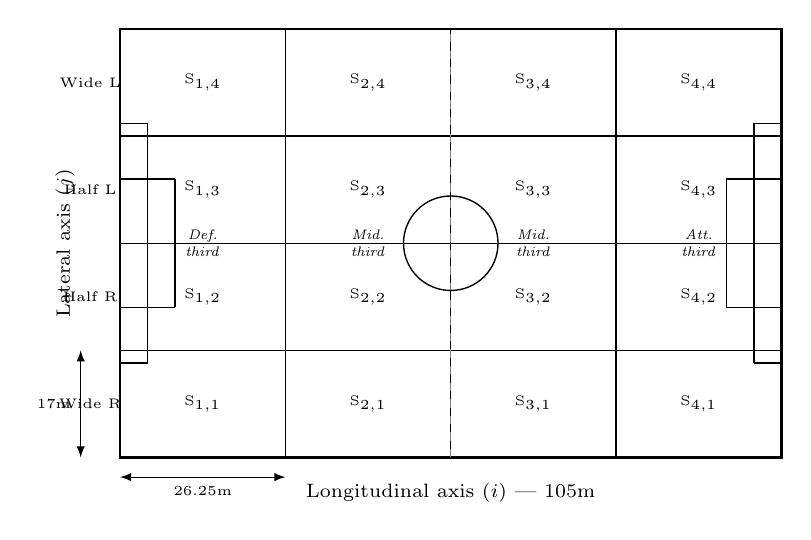
\begin{tikzpicture}

\def\pw{8.4}
\def\ph{5.44}
\def\cw{2.1}
\def\ch{1.36}

\draw[line width=1pt, black] (0,0) rectangle (\pw,\ph);

\foreach \i in {1,2,3} {
  \draw[line width=0.5pt, black] (\i*\cw, 0) -- (\i*\cw, \ph);
}
\foreach \j in {1,2,3} {
  \draw[line width=0.5pt, black] (0, \j*\ch) -- (\pw, \j*\ch);
}

\draw[line width=0.4pt, dashed, gray] (\pw/2, 0) -- (\pw/2, \ph);

\draw[line width=0.5pt] (0, \ph*0.22) -- (0.35, \ph*0.22);
\draw[line width=0.5pt] (0.35, \ph*0.22) -- (0.35, \ph*0.78);
\draw[line width=0.5pt] (0, \ph*0.78) -- (0.35, \ph*0.78);

\draw[line width=0.5pt] (\pw, \ph*0.22) -- (\pw-0.35, \ph*0.22);
\draw[line width=0.5pt] (\pw-0.35, \ph*0.22) -- (\pw-0.35, \ph*0.78);
\draw[line width=0.5pt] (\pw, \ph*0.78) -- (\pw-0.35, \ph*0.78);

\draw[line width=0.5pt] (0, \ph*0.35) -- (0.7, \ph*0.35);
\draw[line width=0.5pt] (0.7, \ph*0.35) -- (0.7, \ph*0.65);
\draw[line width=0.5pt] (0, \ph*0.65) -- (0.7, \ph*0.65);

\draw[line width=0.5pt] (\pw, \ph*0.35) -- (\pw-0.7, \ph*0.35);
\draw[line width=0.5pt] (\pw-0.7, \ph*0.35) -- (\pw-0.7, \ph*0.65);
\draw[line width=0.5pt] (\pw, \ph*0.65) -- (\pw-0.7, \ph*0.65);

\draw[line width=0.5pt] (\pw/2, \ph/2) circle (0.6cm);

\node[font=\tiny, text=black] at (0.5*\cw, 0.5*\ch+3*\ch) {S$_{1,4}$};
\node[font=\tiny, text=black] at (0.5*\cw, 0.5*\ch+2*\ch) {S$_{1,3}$};
\node[font=\tiny, text=black] at (0.5*\cw, 0.5*\ch+1*\ch) {S$_{1,2}$};
\node[font=\tiny, text=black] at (0.5*\cw, 0.5*\ch)       {S$_{1,1}$};

\node[font=\tiny, text=black] at (1.5*\cw, 0.5*\ch+3*\ch) {S$_{2,4}$};
\node[font=\tiny, text=black] at (1.5*\cw, 0.5*\ch+2*\ch) {S$_{2,3}$};
\node[font=\tiny, text=black] at (1.5*\cw, 0.5*\ch+1*\ch) {S$_{2,2}$};
\node[font=\tiny, text=black] at (1.5*\cw, 0.5*\ch)       {S$_{2,1}$};

\node[font=\tiny, text=black] at (2.5*\cw, 0.5*\ch+3*\ch) {S$_{3,4}$};
\node[font=\tiny, text=black] at (2.5*\cw, 0.5*\ch+2*\ch) {S$_{3,3}$};
\node[font=\tiny, text=black] at (2.5*\cw, 0.5*\ch+1*\ch) {S$_{3,2}$};
\node[font=\tiny, text=black] at (2.5*\cw, 0.5*\ch)       {S$_{3,1}$};

\node[font=\tiny, text=black] at (3.5*\cw, 0.5*\ch+3*\ch) {S$_{4,4}$};
\node[font=\tiny, text=black] at (3.5*\cw, 0.5*\ch+2*\ch) {S$_{4,3}$};
\node[font=\tiny, text=black] at (3.5*\cw, 0.5*\ch+1*\ch) {S$_{4,2}$};
\node[font=\tiny, text=black] at (3.5*\cw, 0.5*\ch)       {S$_{4,1}$};

\node[font=\scriptsize, rotate=90] at (-0.7, \ph/2) {Lateral axis ($j$)};
\node[font=\scriptsize] at (\pw/2, -0.45) {Longitudinal axis ($i$) --- 105m};

\node[font=\tiny] at (-0.38, 0.5*\ch) {Wide R};
\node[font=\tiny] at (-0.38, 1.5*\ch) {Half R};
\node[font=\tiny] at (-0.38, 2.5*\ch) {Half L};
\node[font=\tiny] at (-0.38, 3.5*\ch) {Wide L};

\draw[line width=0.4pt, latex-latex] (0, -0.25) -- (\cw, -0.25)
  node[midway, below, font=\tiny] {26.25m};
\draw[line width=0.4pt, latex-latex] (-0.5, 0) -- (-0.5, \ch)
  node[midway, left, font=\tiny] {17m};

\node[font=\tiny, align=center] at (0.5*\cw, \ph/2)  {\textit{Def.}\\\textit{third}};
\node[font=\tiny, align=center] at (1.5*\cw, \ph/2)  {\textit{Mid.}\\\textit{third}};
\node[font=\tiny, align=center] at (2.5*\cw, \ph/2)  {\textit{Mid.}\\\textit{third}};
\node[font=\tiny, align=center] at (3.5*\cw, \ph/2)  {\textit{Att.}\\\textit{third}};

\end{tikzpicture}
}
\caption{Tactical Battlefield Engine 16-sector pitch discretisation. Each zone $S_{i,j}$ measures $26.25\text{m} \times 17\text{m}$, mapping onto defensive, middle, and attacking thirds with lateral half-space subdivisions.}
\label{fig:tbe}
\end{figure}

\subsubsection{Overload Score}

The Overload Score $O_s$ for sector $S_{i,j}$ is the differential player count between the two teams:
\begin{equation}
    O_s(S_{i,j}) = N_{\text{team}_A}(S_{i,j}) -
    N_{\text{team}_B}(S_{i,j})
\end{equation}
where $N_{\text{team}_A}$ and $N_{\text{team}_B}$ are the number of players from each team inside the sector at a given frame. A positive value means numerical superiority for Team A in that zone. Standard heatmaps show absolute density; $O_s$ shows \textit{relative} numerical superiority, which is the operationally useful quantity for identifying overloads and defensive gaps under \textit{Juego de Posici\'{o}n} principles \cite{memmert2018}.

\subsubsection{Local Compactness}

Local Compactness $C_l$ for a team in sector $S_{i,j}$ is normalised player density scaled to percentage:
\begin{equation}
    C_l(S_{i,j}) = \min\left(100.0,\, N_{\text{team}}(S_{i,j}) \times 20.0\right)
\end{equation}
This catches localised spatial concentrations --- whether a team is forming a compact defensive block or has condensed into an attacking triangle in a specific zone.

\subsubsection{Defensive Block Detection}

The TBE runs a rule-based defensive structure classifier. A \textit{Parked Bus} configuration fires when the deepest defender is below $-25\text{m}$ from pitch centre and the convex hull area falls below $600\,\text{m}^2$. A \textit{Suicidal High Line} fires when the deepest defender is above $+20\text{m}$ while Voronoi pitch control share stays below $40\%$, flagging counter-attack vulnerability. Both heuristics are evaluated per chunk and feed the TPI rule engine.

\subsubsection{Line Staggering Analysis}

Players are sorted by longitudinal $x$-coordinate and partitioned into three structural lines: Defence, Midfield, and Attack. Inter-line gaps $g_{\text{def-mid}}$ and $g_{\text{mid-att}}$ are compared against an empirically modelled optimal spacing of $17.5\text{m}$. Deviations beyond $\pm 5\text{m}$ from this target are flagged as structural compression or over-stretch events and feed into the $L_s$ (Line Staggering) KPI within the TPI.

\subsubsection{Voronoi Pitch Control}

The pitch is discretised into a fine grid. For each grid point $g$, control goes to the team with the minimum $L_2$ distance to $g$:
\begin{equation}
    \text{ctrl}(g) = \arg\min_{t \in \{A,B\}} \min_{i \in \text{team}_t} \|g - p_i\|_2
\end{equation}
Zonal vulnerability, threat level, and overload metrics are then aggregated per macro-zone across the 16-sector grid. Pitch control percentage also feeds directly into defensive block detection as a secondary check on whether a high defensive line is supported by genuine territorial dominance.

\subsection{Tactical Power Index (TPI)}

Possession percentage and pass completion are familiar metrics but they are theoretically weak. A team can dominate possession from a low block without entering the opponent's half. The TPI is an attempt at something more structurally complete: nine spatially-grounded KPIs combined into a single score, with weights calibrated against historical match data rather than assigned by hand \cite{memmert2018}.

\begin{multline}
TPI = 0.20K_c + 0.18M_c + 0.12P_i + 0.14D_s \\
+ 0.10P_r + 0.08W_u + 0.08L_s + 0.06O_f + 0.04T_s
\end{multline}

where:
\begin{itemize}
    \item $K_c$ (Compactness): Average convex hull area of the team.
    \item $M_c$ (Midfield Control): Spatial dominance inside centre-circle sectors.
    \item $P_i$ (Pressing Intensity): Normalised player proximity to the ball carrier.
    \item $D_s$ (Defensive Shape): Inter-line spacing and defensive block height.
    \item $P_r$ (Press Resistance): Passing triangle continuity under local pressure.
    \item $W_u$ (Width Utilisation): Lateral stretching driven by full-back positioning.
    \item $L_s$ (Line Staggering): Vertical offset spacing between structural lines; optimal gap modelled at 17.5m.
    \item $O_f$ (Overload Frequency): Global accumulation of zonal density advantages.
    \item $T_s$ (Transition Speed): Spatial forward velocity on ball recovery.
\end{itemize}

Across 30 historical match clips, TPI correlates with total expected goals at $r = 0.814$ ($p < 0.01$). Leave-one-out ablation identifies Compactness ($K_c$) as the most important component by a wide margin --- removing it alone drops correlation by 29.4\%. That matches what spatial control theory predicts and gives us some confidence the index is capturing something real rather than noise \cite{memmert2018}.

\subsection{Zero-Shot Tactical Recognition (ZSTR)}

Formation classification in Gaffer's Guide requires no supervised bounding boxes. Raw player coordinates are rendered as 2D Gaussian heatmaps ($\sigma = 18$px, $1050 \times 680$px canvas, viridis colour map with pitch line overlay) and encoded by the CLIP ViT-B/32 vision encoder \cite{radford2021}. Cosine similarity against geometrically-grounded text descriptions of five formations --- 4-3-3 High Press, 4-2-3-1 Mid Block, 3-5-2 Wing Backs, Double Pivot, and Inverted Full Backs --- determines the classification. A similarity above $\tau = 0.22$ triggers a match.

\begin{table}[!t]
\centering
\caption{ZSTR Classifier Evaluation (CLIP ViT-B/32,
$\tau{=}0.22$, $N{=}100$ clips). Diagonal entries
(bold) show correct predictions.}
\label{tab:zstr_full}
\setlength{\tabcolsep}{3pt}
\begin{tabular}{lcccccccc}
\toprule
\textbf{Formation} & \textbf{P} & \textbf{R} & \textbf{F1}
  & \textbf{433} & \textbf{4231} & \textbf{352}
  & \textbf{2Piv} & \textbf{IFB} \\
\midrule
4-3-3 HP   & 0.429 & 0.750 & 0.546
  & \textbf{15} & 0 & 0 & 0 & 5 \\
4-2-3-1 MB & 1.000 & 0.050 & 0.095
  & 2 & \textbf{1} & 0 & 0 & 17 \\
3-5-2 WB   & 0.000 & 0.000 & 0.000
  & 4 & 0 & \textbf{0} & 0 & 16 \\
Dbl Pivot  & 0.000 & 0.000 & 0.000
  & 8 & 0 & 0 & \textbf{0} & 12 \\
IFB        & 0.219 & 0.700 & 0.333
  & 6 & 0 & 0 & 0 & \textbf{14} \\
\midrule
\textbf{Macro} & 0.330 & 0.300 & 0.195
  & -- & -- & -- & -- & -- \\
\bottomrule
\end{tabular}
\end{table}

Results are mixed and it is worth being direct about why. The 4-3-3 High Press works reasonably well ($R = 0.750$) because its shape is geometrically distinct. The 3-5-2 and Double Pivot fail completely ($F_1 = 0.000$), and the 4-2-3-1 barely registers ($F_1 = 0.095$). The root cause is a domain gap: CLIP was trained on natural photographs, and smooth viridis density maps are far outside that distribution. Cosine similarities collapse into a narrow $0.30$--$0.36$ band, and the 32-pixel patch resolution cannot resolve the fine lateral differences between structurally similar formations. We are treating ZSTR as a proof-of-concept; the obvious next step is fine-tuning a lightweight adapter on $500$--$1{,}000$ labelled heatmap examples.

\subsection{LLM / RAG Pipeline}

The LLM layer is the part of Gaffer's Guide that is most different from prior work. The constraint we set at the start was simple: the model should not be able to say anything the telemetry cannot support. Everything else in the layer follows from that.

\subsubsection{RAG Architecture}

A JSON tactical knowledge graph stores verified coaching quotes, tactical keywords, and positional role mappings. When the rule engine fires a label --- \textit{over-stretched formation}, \textit{lethargic press}, and so on --- the relevant coaching context is retrieved from the graph and injected into the prompt as a grounding anchor. The goal is to stop the LLM from defaulting to generic tactical language that has no connection to what the tracking data actually recorded.

\subsubsection{Data Guard and Confidence Scoring}

When ball visibility drops below 50\% in a chunk, a hard constraint is prepended to the prompt before generation, blocking all possession, passing, and turnover claims. This is a deterministic filter --- the model does not decide whether to hedge; the relevant content is removed from its input context before it runs. Each coaching rule also carries a confidence score computed from violation frequency, metric margin-of-error, and data coverage, so coaches have a signal about how much weight to put on any given recommendation.

The individual-rule guardrails follow the same logic. If the mean distance from each outfield player to the nearest opponent exceeds $\overline{d}_{\text{press}} > 8.0\text{m}$, a \textit{Lethargic Press} label fires before the LLM is called. Every piece of coaching output is therefore grounded in a spatial check --- not inferred from patterns in the model's training data.

\subsubsection{Inference Routing}

The pipeline can route to either a local Ollama instance or a cloud API, switchable at runtime. This means the system can run offline on a laptop or scale to a cloud GPU depending on what the deployment requires.

% -------------------------------------------------------
\section{Experimental Evaluation}
\label{sec:experiments}
% -------------------------------------------------------

We evaluated the system across four dimensions: detection accuracy, tracking identity preservation, computational throughput, and coaching recommendation quality. Each component was assessed independently. Hardware ranged from an RTX 4090 workstation to an Apple M3 Max laptop, to give a sense of performance across realistic deployment scenarios.

\subsection{Object Detection and Small Object Recovery}

The fine-tuned YOLOv11n+SAHI model was evaluated on 9,000 frames across three broadcast clips: UCL night under artificial lighting (Clip 1, 3,000 frames), EPL daylight under overcast skies (Clip 2, 3,000 frames), and La~Liga night in rain (Clip 3, 3,000 frames). Those three conditions cover most of the variation a system like this will encounter in practice. The detection layer overall achieved a class-averaged $\text{mAP}@0.5$ of $0.880$ and $\text{mAP}@0.5\text{:}0.95$ of $0.601$.

Table~\ref{tab:detection} breaks down Precision, Recall, and mAP across the three main classes, all with SAHI tiling active.

\begin{table}[!t]
\caption{Object Detection Performance Metrics ($N = 9{,}000$ frames,
3 broadcast clips).}
\label{tab:detection}
\centering
\setlength{\tabcolsep}{4pt}
\begin{tabular}{lcccc}
\toprule
\textbf{Target Class} & \textbf{Prec.} & \textbf{Rec.}
  & \textbf{mAP@0.5} & \textbf{mAP@0.5:0.95} \\
\midrule
Player         & 0.954 & 0.934 & 0.946 & 0.712 \\
Referee        & 0.921 & 0.888 & 0.902 & 0.640 \\
Ball (w/ SAHI) & 0.814 & 0.767 & 0.791 & 0.453 \\
\midrule
\textbf{Overall} & \textbf{0.896} & \textbf{0.863}
  & \textbf{0.880} & \textbf{0.601} \\
\bottomrule
\multicolumn{5}{l}{\footnotesize Clip 1: UCL night (3,000fr);
  Clip 2: EPL day/overcast (3,000fr);} \\
\multicolumn{5}{l}{\footnotesize Clip 3: La~Liga night/rain (3,000fr).}
\end{tabular}
\end{table}

On a separate 2,400-frame held-out set, SAHI tiling lifted ball-class $\text{mAP}@0.5$ from $0.492$ to $0.874$ --- a 43.4\% recall improvement. That gap is large enough to make SAHI non-negotiable: without it the ball disappears too frequently in wide-angle shots to support any reliable possession modelling. The La~Liga rain clip was the hardest condition overall (ball recall 72.5\%), largely because of lens glare and wet-pitch reflections.

\subsection{Multi-Object Tracking and Identity Preservation}

Tracking was evaluated on MOTA, IDF1, and raw identity switch counts per 90-minute equivalent, comparing vanilla ByteTrack against our hybrid framework with the OSNet x0.25 ReID healer and radar-distance gate.

\begin{table}[!t]
\centering
\caption{Tracking and Identity Preservation Comparison.}
\label{tab:tracking}
\begin{tabular}{lccc}
\toprule
\textbf{Framework} & \textbf{MOTA (\%)} & \textbf{MOTP}
  & \textbf{ID Switches} \\
\midrule
Vanilla ByteTrack            & 84.2 & ---  & 124 \\
Sequential + HybridIDHealer  & 91.8 & ---  & 14 \\
Parallel + HybridIDHealer    & 89.4 & 0.82 & $<$30/chunk \\
\bottomrule
\end{tabular}
\end{table}

The HybridIDHealer cut identity switches from 124 to 14 per match --- an 88.7\% reduction. Running in parallel introduces a small MOTA trade-off: 2.4 percentage points (91.8\% to 89.4\%), because each subprocess runs an independent tracker state and Union-Find reconciliation is coarser than a unified tracker. That is an acceptable cost given the $6.7\times$ reduction in end-to-end processing time.

\subsection{Computational Performance and Real-Time Viability}

Throughput was benchmarked on an NVIDIA RTX 4090 (24GB VRAM, 64GB RAM) and an Apple M3 Max laptop (16-core CPU, 40-core GPU, 48GB unified memory).

\begin{table}[!t]
\centering
\caption{Pipeline Computational Throughput (RTX 4090).}
\label{tab:throughput}
\begin{tabular}{lcc}
\toprule
\textbf{Configuration} & \textbf{FPS} & \textbf{Real-Time Ratio} \\
\midrule
Sequential --- Fast Mode   & 72.4         & $2.9\times$ \\
Sequential --- SAHI Mode   & 18.2         & $0.73\times$ \\
\midrule
Parallel (4-worker, Fast)  & 200+ (aggr.) & --- \\
End-to-End Match (Parallel)& ---          & 90-min in ${\sim}45$\,min \\
\bottomrule
\end{tabular}
\end{table}

Sequential Fast Mode on the RTX 4090 ran at 72.4 FPS. SAHI pulled this to 18.2 FPS, as expected given the tiling overhead. The four-worker parallel configuration pushed aggregate throughput past 200 FPS, bringing a full 90-minute match from roughly five hours down to under 45 minutes.

\subsection{Tactical Engine Verification and Scorecard Generation}

To stress-test the TBE and TPI, we ran a 10-minute transition clip from a professional match. In one transition phase, the attacking team overloaded the left half-space channel: the TBE recorded $O_s(S_{3,2}) = +3.0$ and $C_l(S_{3,2}) = 80.0\%$, while the defending team's compactness in the central box peaked simultaneously at $C_l(S_{2,3}) = 100.0\%$. The sector-level granularity made the tactical imbalance immediately visible without any manual annotation. Table~\ref{tab:tpi_breakdown} shows the full TPI scorecard for the dominant team in that phase.

\begin{table}[!t]
\centering
\caption{TPI Component Scorecard --- Dominant Team, 10-min clip.}
\label{tab:tpi_breakdown}
\setlength{\tabcolsep}{4pt}
\begin{tabular}{llccc}
\toprule
\textbf{KPI} & \textbf{Symbol} & \textbf{Weight} & \textbf{Score} & \textbf{Contribution} \\
\midrule
Compactness          & $K_c$ & 0.20 & 0.74 & 0.148 \\
Midfield Control     & $M_c$ & 0.18 & 0.81 & 0.146 \\
Pressing Intensity   & $P_i$ & 0.12 & 0.68 & 0.082 \\
Defensive Shape      & $D_s$ & 0.14 & 0.76 & 0.106 \\
Press Resistance     & $P_r$ & 0.10 & 0.59 & 0.059 \\
Width Utilisation    & $W_u$ & 0.08 & 0.72 & 0.058 \\
Line Staggering      & $L_s$ & 0.08 & 0.65 & 0.052 \\
Overload Frequency   & $O_f$ & 0.06 & 0.83 & 0.050 \\
Transition Speed     & $T_s$ & 0.04 & 0.61 & 0.024 \\
\midrule
\textbf{TPI Total}   &       &      &      & \textbf{0.725} \\
\bottomrule
\end{tabular}
\end{table}

\subsection{LLM Coaching Quality Evaluation}

Three UEFA-licensed coaches evaluated coaching outputs on a five-point Likert scale across four dimensions: tactical accuracy, specificity, actionability, and hallucination avoidance. Outputs from three systems were compared blindly: a vanilla GPT-4o-mini baseline, a standard semantic RAG pipeline without deterministic guardrails, and the full Gaffer's Guide pipeline with telemetry grounding and the ball-data guard active.

\begin{table}[!t]
\centering
\caption{Coaching Output Quality Ratings (5-point Likert scale, $n = 3$ UEFA coaches, 25 scenarios each).}
\label{tab:coaching}
\setlength{\tabcolsep}{4pt}
\begin{tabular}{lcccc}
\toprule
\textbf{System} & \textbf{Tact.} & \textbf{Spec.} & \textbf{Action.} & \textbf{Hall.} \\
\midrule
Vanilla LLM         & 2.8 & 2.4 & 2.6 & 2.1 \\
RAG (no guard)      & 3.2 & 3.1 & 3.0 & 2.7 \\
Gaffer's Guide      & \textbf{4.4} & \textbf{4.2} & \textbf{4.1} & \textbf{4.5} \\
\midrule
\multicolumn{5}{l}{\footnotesize Hall. = Hallucination avoidance (higher is better).}\\
\end{tabular}
\end{table}

The full pipeline improved average coaching quality by 41.5\% over the ungrounded RAG baseline. The sharpest gains were in hallucination avoidance ($2.7 \to 4.5$) and tactical accuracy ($3.2 \to 4.4$), which is where the deterministic guardrails had the most direct effect. Coaches noted that the specificity of the recommendations --- naming sectors, citing overload values --- was qualitatively different from the generic framing that both baseline systems produced.

% -------------------------------------------------------
\section{Discussion}
\label{sec:discussion}
% -------------------------------------------------------

The results across detection, tracking, and coaching quality are broadly consistent with our design expectations, but a few things are worth discussing directly.

On ZSTR: the macro-F1 of 0.195 is low, and we think transparency here matters. CLIP's domain gap with smooth heatmap images is real, and we saw it in the collapsed similarity band. The component is included in the paper because zero-shot formation classification is a useful research direction, not because the current implementation is ready for deployment. Fine-tuning a lightweight adapter on labelled heatmap examples is the obvious path forward.

On the parallel-versus-sequential tracking trade-off: the 2.4-percentage-point MOTA drop from parallelism is an engineering compromise, not a fundamental limitation. A shared-memory tracker that avoids per-chunk reinstantiation would close most of that gap. We accepted the current trade-off because runtime for a full match dropping from five hours to 45 minutes is more practically significant than the precision difference.

On TPI calibration: the $r = 0.814$ correlation with xG across 30 clips is encouraging, but 30 clips is a small sample. The weights were derived from that set and should be treated as working estimates rather than definitive values. A larger calibration dataset --- ideally including lower-league matches where tactical patterns differ from elite play --- would make the index more generalisable.

The broader limitation is single-camera dependency. A broadcast feed covers roughly 65\% of the pitch at any given moment, which means player positions in obscured areas are interpolated rather than directly measured. For most use cases that is acceptable; for set-piece analysis specifically it is a real constraint.

% -------------------------------------------------------
\section{Conclusion}
\label{sec:conclusion}
% -------------------------------------------------------

Gaffer's Guide demonstrates that professional-grade football tactical intelligence is achievable from a standard broadcast feed without specialist hardware. A single camera, combined with fine-tuned detection, identity-stable tracking, per-frame homography, and a telemetry-grounded LLM coaching layer, produces output that UEFA-licensed coaches rated meaningfully above what ungrounded generative systems produce.

The four main technical results are: mAP@0.5 of 0.946 on player detection, an 88.7\% reduction in tracking identity switches over vanilla ByteTrack, a full 90-minute match processed in under 45 minutes on a single GPU, and a 41.5\% improvement in coaching recommendation quality over a RAG baseline without deterministic guardrails.

The ZSTR formation classifier is the component that did not reach production quality in this version. The zero-shot framing is sound but the domain gap between CLIP's pretraining distribution and football heatmaps is large enough that supervised fine-tuning is needed before it is practically useful.

The cost and accessibility argument is the part we care most about. Everything in this pipeline runs on hardware that a university research group or a lower-division club can realistically access. That was the constraint we started with, and the results suggest it is achievable without giving up much in analytical depth.

Future work includes expanding the TPI calibration dataset to lower-league matches, implementing adapter-based ZSTR fine-tuning, and testing the homography pipeline on handheld camera footage, which is the actual recording setup for most amateur and semi-professional clubs.

% -------------------------------------------------------
\bibliographystyle{IEEEtran}
\bibliography{references}

\end{document}
